\chapter{System Design}
\label{chap:systemDesign}
In this chapter, we will describe the software architecture of the applications.
We will focus on high level abstractions of the system. More detailed class diagrams of the system
is found in Appendix \ref{chap:class-diagram}.

\section{Architectural Description}

This project is a prototype to test a concept based
on gamification on asthma-treatments. Thus, the main architectural qualities 
identified for the applications is modifiability and usability. 
The reasoning behind this decision is that the software should be easy to modify with extended 
functionality if the concept is proven successful. 
It should
also be intuitive to use, since many of our potential users are children at ages below eight years old. Usability is our top priority.


We chose Model-View-Controller (MVC) as the architectural pattern for GAPP and CAPP, as MVC seperates the
underlying data models from views, and is proven to enhance modifibility. 
It is also an integrated part in Android, through a class called \code{Activity}.
We will explain more about activities in Section \ref{sec:gapp-dev-view}.
  



\section{Software architecture}
\emph{``The Software Architecture of a program or computing system is the structure or structures of the system, which comprise
software elements, the externally visible properties of those elements, and the relationships among them.''} \cite{bassclemetskazman}.
 
In the following section, we will describe the architecture of the system according to the 4+1 View Model 
introduced in Section \ref{sec:viewmodel}.


The relevant stakeholders for the architecture is NAAF, Sykehusapotekene
i Midt-Norge, NTNU, in addition to future and present developers. In this section, we will
describe the architecture of the system through a Logical View, Development
View and a Process View. We have not created a Physical View, a this is not usual for a software that does not run on some sort of special hardware. 
The different views build upon the use cases defined in Section \ref{sec:useCases}


\clearpage{}
\subsection{Logical View}
\label{sec:logical-view-parent}
The purpose of the Logical View is to give interested stakeholders an overview of the different modules of the system, 
and how they communicate between each other. 
   

\begin{figure}
	\centering
		\includegraphics[width = 11.5 cm]{Pictures/ArchPictures/logicview.png}
	\caption{Logical View for the system} 
	\label{fig:package-diagram-system}
\end{figure}

Figure \ref{fig:package-diagram-system} shows the package diagram for the system. 

The locial view shows the different modules of the system, and the communication protocols between them. 


As mentioned in Section \ref{sec:pollencast}, NAAF provides a pollen forecast at \url{http://pollenvarslingen.no} which we intended to integrate with our system. It is currently not connected,
because the pollen forecast only operates during pollen season. It is however an important component for GAPP, and should be put in use during further development. 
We have worked around this fact in order to give the prototype a bit more content. This is described in more details in Appendix \ref{chap:class-diagram}.
 

The webservice is an important part that ties the different applications together. It required a lot of hours spent on developing it during the early stages, but
it definetly paid off later. 
There were several reasons to provide a webservice for the application:
\begin{itemize}
  \item Karotz only provides HTTP GET and POST methods for communicating over network,
  \item Our database server allocated at mysql.stud.ntnu.no is only available from NTNU's LAN (Local area network), which in practice means that a phone that is not connected to eduroam would get access to the database. 
  \item All MySQL queries are allocated at the same place.
\end{itemize}


% This package diagram is the top level folder structure for GAPP. Since we are using a MySQL-database hosted at NTNU, we had to work around
% some problems considering that we don't have access to the database unless we are connected to NTNU's LAN. The solution to this problem 
% introduced the webservice, which serves the purpose as a middle man between GAPP and the database. From this webservice, we retrieve data from over HTTP,
% using JSON. We also post data to the database through the package called jsonposters. Note that there is no security in this webservice, 
% which needs to be changed before deployment.
%  
% The diagram also shows a package called xmlfeed. This package serves the purpose of parsing XML into Java-code. Originally, the idea was to
% use pollenvarslingen.no's XML-feed. However, this feed is not running at the autumn and winter, so we replicated that XML-feed in our own 
% ``dummy''-feed \footnote{This XML-file is hosted at: \url{http://folk.ntnu.no/yngvesva/blopp/dummy/PollenForecast.xml}}.
% 
% This xml-document has similar structure as the original feed, only with test data for the sake of the prototype and proof-of-concept. 
% We have developed GAPP using MVC as our main architectural pattern. However, implementing MVC in Android is a bit different from other applications. 
% In Android, the activities serves both as a View and as the Controller (because of the touch screen).
% Thus, the Activity package will include all Activities needed, like \code{MainMenu} and \code{DistractionActivity}, etc. In addition, in order to render listviews, gridviews, etc.
% we need to make custom adapters, hence introducting the adapters-package. 
% 
% The package views only contains the relevant classes for the Log. We need this package since \code{CalendarView} is rendered programatically (taking
% dates into consideration when rendering). 
% 
% The repositories-package is not used at the moment, but we figured it would be a good idea to introduce it here for the future development team. Before the system is deployed,
% we expect that the database server will be changed. The repositories-package is a brief start on which functionality that needs to be implemented if the application
% is going to communicate directly with the database. It is by no means ready to put in use, but it is a start.   
% 
% We'll explain the content in each package more detailed in the Development View.
% 
% \subsubsection{Logical View -- CAPP}
% \begin{figure}
% 	\centering
% 		\includegraphics[width = 11.5 cm]{Pictures/ArchPictures/capparchpictures/capp_package_diagram}
% 	\caption[GAPP package diagram]{Package diagram for CAPP. A line from package X to package Y describes an association from X to Y. }
% 	
% 	\label{fig:package-diagram-system-capp}
% \end{figure}
% 
% Figure \ref {fig:package-diagram-system-capp} shows the logical view (package diagram) for CAPP. CAPP has about the same architecture as GAPP. 
% The main difference is the ``services'' package. A service in Android is a task that is done without any interactions from the user. In our case, 
% we use the services-package to update alarms once the phone is turned on, and on request. CAPP uses the same database and webservice as GAPP, and 
% a lot of the parsers in this application are equal to those found in GAPP.
% 
% \subsubsection{Logical View -- Karotz}
%  \begin{figure}
%  	\centering
%  		\includegraphics[width=12cm]{Pictures/ArchPictures/KarotzPackageDiagram}
% 	\caption[Karotz package diagram]{Package diagram for the Karotz application}
% 	\label{fig:package-diagram-system-karotz}
%  \end{figure}
% 
% Figure \ref{fig:package-diagram-system-karotz} shows the logical view of the Kartoz application. The only internal package in the Karotz application 
% is named ``src''. It contains all the main logic for the application, including a repository for connecting to the webservice for connecting to the 
% database, a notification module for setting alarms, a medication module for doing distraction; and a ``Blopp'' module for keeping track of everything. 
% There is an additional package in the diagram named ``\lbrack{}static\rbrack{}''. It contains the Karots class which is inherited from the OS and 
% contains various utilities for controlling output and recieveing input for the robot. It has been extended with some helper methods in the 
% implementation. There is also a ``util'' class which contains additional utility methods that do not belong in ``Karotz''. At last, there is indicated 
% an ``External'' package, which symbolizes all the external services the application connects to. In the case of the Karotz application, this includes 
% only the web service that connects to the database.
\subsection{Development View}

Our development view is represented through a package diagram, and gives a brief overview of the different packages implemented in GAPP and CAPP. 
We have implemented somewhere around 120 different Java classes, which does not include the Karotz code. 

\subsubsection{Development View -- GAPP}
\label{sec:gapp-dev-view}

\begin{figure}
	\centering
		\includegraphics[width = 11.5 cm]{Pictures/ArchPictures/gapparchpictures/gapp_package_diagram.png}
	\caption[GAPP package diagram]{Package diagram for GAPP. A line from package X to package Y describes an association from X to Y. }
	\label{fig:package-diagram-gapp}
\end{figure}

Figure \ref{fig:package-diagram-gapp} show the top level package structure for GAPP. In the logical view, we introduced our webservice. 
From this webservice, we retrieve data over HTTP GET,
using JSON (JavaScript Object Notation). The classes found in jsonposters uses HTTP POST to send data to the webservice, which in turn forwards the information sent to our database. 

The diagram also shows a package called xmlfeed. This package serves the purpose of parsing XML (Extensible Markup Language) into Java-code. Originally, the idea was to
use NAAF's XML-feed. However, this feed is not running during autumn and winter, so we replicated that XML-feed in our own
``dummy''-feed \footnote{This XML-file is hosted at: \url{http://folk.ntnu.no/yngvesva/blopp/dummy/PollenForecast.xml}}. 
This xml-document has similar structure as the original feed, only with test data for the sake of the prototype and proof-of-concept.

The package activities contains classes that extends \code{Activity}, which is an android class that functions as both the View and Controller in MVC. 
An example of an implemented activity is \code{MainMenu}.

In order to render listviews and gridviews programatically, we needed to make a package called adapters. An \code{Adapter} in Android serves the purpose of filling  
these list- and gridviews with data.
 
Views in Android can be created in two ways. Either through an XML layout file, or by customising in Java. Most of our views are using XML-files. We have one custom
made view (\code{CalendarView}, used to implement our logging functionality), which is available in the package ``views''. 
The XML-files are not shown in this diagram, but is included in the application's resource folder, which is standard when working
in the Android framework.  
  

We'll explain the content in each package more detailed in the Development View.

\subsubsection{Development View -- CAPP}
\begin{figure}
	\centering
		\includegraphics[width = 11.5 cm]{Pictures/ArchPictures/capparchpictures/capp_package_diagram}
	\caption[GAPP package diagram]{Package diagram for CAPP. A line from package X to package Y describes an association from X to Y. }

	\label{fig:package-diagram-system-capp}
\end{figure}

Figure \ref {fig:package-diagram-system-capp} shows the package diagram for CAPP. CAPP has very similar architecture as GAPP.
The main difference is the ``services'' package. A service in Android is a task that is executed without any interactions from the user. In our case,
we use the services-package to update alarms. CAPP uses the same database and webservice as GAPP, and
a lot of the parsers in this application are equal to those found in GAPP.

\subsubsection{Development View -- Karotz}
 \begin{figure}
 	\centering
 		\includegraphics[width=12cm]{Pictures/ArchPictures/KarotzPackageDiagram}
	\caption[Karotz package diagram]{Package diagram for the Karotz application}
	\label{fig:package-diagram-system-karotz}
 \end{figure}

Figure \ref{fig:package-diagram-system-karotz} shows the development view of the Kartoz application. The only internal package in the Karotz application
is named ``src''. It contains all the main logic for the application, including a repository for connecting to the webservice for connecting to the
database, a notification module for setting alarms, a medication module for doing distraction, and a ``Blopp'' module for keeping track of everything.
There is an additional package in the diagram named ``\lbrack{}static\rbrack{}''. It contains the Karots class which is inherited from the OS and
contains various utilities for controlling output and recieveing input for the robot. It has been extended with some helper methods in the
implementation. There is also a ``util'' class which contains additional utility methods that do not belong in ``Karotz''. At last, there is indicated
an ``External'' package, which symbolizes all the external services the application connects to. In the case of the Karotz application, this includes
only the web service that connects to the database.

\subsection{Process View}
\label{sec:processView}
The purpose of the Process View is to give the customer an overview of how some
of the main functionality has been implemented. We have chosen to do this
through Sequence Diagrams. These diagrams shows the main data flow of the system.

We have chosen to include the following functionality:
\begin{itemize}
	\item Medication completed
	\item Change of childrens health status
\end{itemize}



\subsubsection{Medication Completed}
\begin{figure}[h!]
	\centering
		\includegraphics[width = 17.5 cm]{Pictures/ArchPictures/gapparchpictures/medication_finished.png}
	\caption{Sequence diagram for medication completed}
	\label{fig:seq-diagram-medication}
\end{figure}

Figure \ref{fig:seq-diagram-medication} shows a sequence diagram for the event of a medication completed. 
When a medication is completed, \code{DistractionActivity} creates a new instance of \code{RegisterMedicinePostModel}, before it uses this instance's \code{toString()} method to 
create an instance of \code{PostRegisterTreatment}. This poster does an HTTP POST to ``register\_medicine\_taken.php'', which 
in turn updates the databse. The webservice then returns JSON-formatted data, with the reward included. \code{RegisterMedicinePostModel} 
interprets the returned data, and stores the reward in a private variable, which the \code{DistractionActivity} in turn accesses to show the 
child the reward collected from the treatment.

\subsubsection{Change Of Childrens Health Status}
\begin{figure}[h!]
	\centering
		\includegraphics[width = 17.5 cm]{Pictures/ArchPictures/gapparchpictures/sequence_health_state.png}
	\caption{Sequence diagram for changing medication plan}
	\label{fig:seq-diagram-healthstate}
\end{figure}
Figure \ref{fig:seq-diagram-healthstate} shows a sequence diagram for the event of changing
a child's health status. The user gives input on one of three checkboxes that \code{MedicationPlanActivity} receives. The activity then calls creates 
a new instance of \code{HealthStatePostModel}, and uses this model's \code{toString()} to execute \code{HealthStatePoster}. \code{HealthStatePoster} makes an HTTP POST to ``set\_child\_state.php'' with 
appropriate POST parameters. The webservice updates the database, before it returns JSON-formatted data to the \code{HealthStatePoster}.

\subsubsection{Notification and medication on Karotz}
\begin{figure}
	\centering
		\includegraphics[width=\linewidth]{Pictures/ArchPictures/KarotzMedicationSequence}
	\caption{Sequence diagram for notification and medication on Karotz}
	\label{fig:karotz-sequence}
\end{figure}
Figure \ref{fig:karotz-sequence} shows a sequence diagram for notification and medication on the Karotz. The Karotz routinely updates itself by
calling a get function on the database access layer. The \code{Repository} object requests that a new notification event is made for the closest
medicine dose that should be taken. When the timeout is done, \code{Notification} calls \code{startMedication()} in \code{Medication} in order
to start a sequence of events that makes up the distraction sequence. This sequence is represented as a list of actions---called a \emph{manuscript}.
The manuscript is interpreted by the \code{util} module which creates and runs a function based on a premade specification. Each action contains
an url to a sound file, and an activator which represents how the next action in the manuscript is triggered. The manuscript is detailed further in
Appendix \ref{apx:karotzManuscript}. When each action in the manuscript is completed, the \code{Medication} module calls \code{logMedicineTaken()}
in \code{Repository} once for each dose, and the database is thus updated with the registered medicines.


\clearpage{}
\section{Architecture Rationale}

Choosing MVC has become a somewhat ``standard'' solution for these types of applications, and it was a successful pattern for our use as well.   
The choice of making the database accessible through a webservice slowed down performance a bit, but we had to do this, since Karotz only
supports access to the database through the webservice. 
We were also not able to implement proper caching functionality, which could have improved performance severly. More information on this part
is found in Chapter \ref{chap:furtherWork}. 

We found it somewhat harder to implement good models 
for the objects that is retrieved from the webservice, which has created a bit of overhead in the architecture.
However, it has been easier to connect CAPP and GAPP together by retrieving data
through the same webservice, and it was a working solution once we knew how to access it properly. 


It is hard to predict how many users the system can handle once proper functionality for several children is implemented. 
The webservice is developed with the intention of running at one server only, and so, the scalability of the system 
is very dependent
on the capabilties of this server (how many requests it can handle per time unit). If the software is to be depolyed on 
several servers, the webservice needs to be rewritten. 

\section{Database}
The database implementation is based on an ER (entity relationship) diagram, which is illustrated in the
diagram in section \ref{sec:databaseImplementaion}. It is created based on the 
final implementation. There is also a separate access layer for modifying and 
viewing the data through the web.

%\subsection{ER diagram for the database}
Figure \ref{fig:db-er-diagram} shows an ER diagram of the structures and relationships
of the tables in the database.

\begin{landscape}
\begin{figure}
% 	\vspace{-4cm}
	\centering
		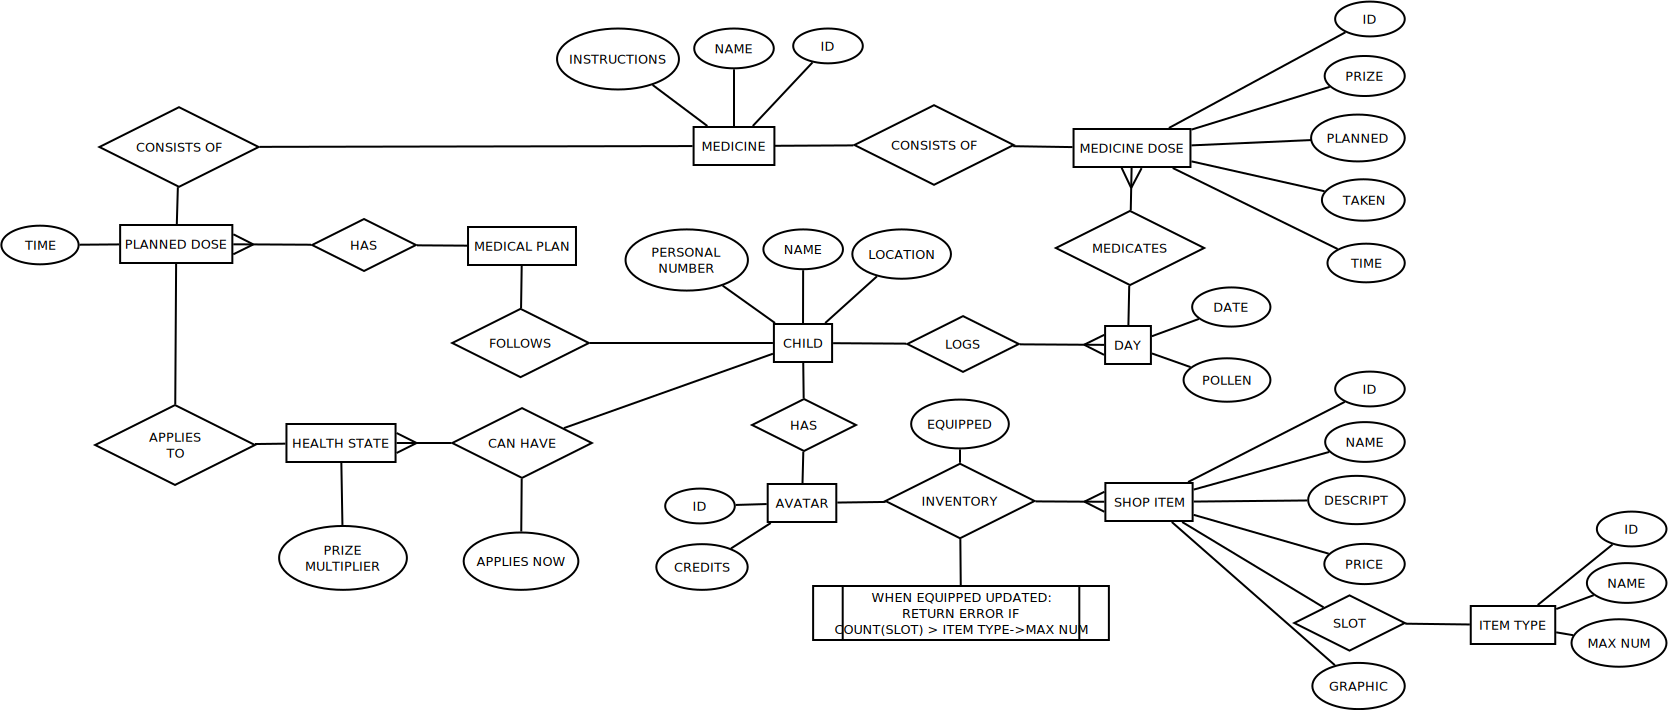
\includegraphics[width=0.9\paperheight]{Pictures/ArchPictures/BLOPP_DB_ER_diagram.png}
	\caption{ER diagram for the BLOPP database}
	\label{fig:db-er-diagram}
\end{figure}
\end{landscape}
%\subsection{Database \LaTeX{} export for database}
% phpMyAdmin LaTeX Dump
% version 2.5.6
% http://www.phpmyadmin.net
%
% Host: mysql.stud.ntnu.no
% Generation Time: Sep 12, 2012 at 09:14 AM
% Server version: 5.0.96
% PHP Version: 5.2.4-2ubuntu5.25
% 
% Database : `yngvesva_blopp`
% 

%
% Structure: AVATARS
%
 \begin{longtable}{|l|c|c|c|} 
 \caption{Structure of table AVATARS} \label{tab:AVATARS-structure} \\
 \hline \multicolumn{1}{|c|}{\textbf{Field}} & \multicolumn{1}{|c|}{\textbf{Type}} & \multicolumn{1}{|c|}{\textbf{Null}} & \multicolumn{1}{|c|}{\textbf{Default}} \\ \hline \hline
\endfirsthead
 \caption{Structure of table AVATARS (continued)} \\ 
 \hline \multicolumn{1}{|c|}{\textbf{Field}} & \multicolumn{1}{|c|}{\textbf{Type}} & \multicolumn{1}{|c|}{\textbf{Null}} & \multicolumn{1}{|c|}{\textbf{Default}} \\ \hline \hline \endhead \endfoot \textbf{\textit{id}} & int(11) & Yes & NULL \\ \hline 
credits & int(11) & Yes & 0 \\ \hline 
\textbf{inventory\_id} & int(11) & Yes & NULL \\ \hline 
 \end{longtable}

%
% Structure: AVATAR_INVENTORIES
%
 \begin{longtable}{|l|c|c|c|} 
 \caption{Structure of table AVATAR\_INVENTORIES} \label{tab:AVATAR_INVENTORIES-structure} \\
 \hline \multicolumn{1}{|c|}{\textbf{Field}} & \multicolumn{1}{|c|}{\textbf{Type}} & \multicolumn{1}{|c|}{\textbf{Null}} & \multicolumn{1}{|c|}{\textbf{Default}} \\ \hline \hline
\endfirsthead
 \caption{Structure of table AVATAR\_INVENTORIES (continued)} \\ 
 \hline \multicolumn{1}{|c|}{\textbf{Field}} & \multicolumn{1}{|c|}{\textbf{Type}} & \multicolumn{1}{|c|}{\textbf{Null}} & \multicolumn{1}{|c|}{\textbf{Default}} \\ \hline \hline \endhead \endfoot \textbf{\textit{id}} & int(11) & Yes & 0 \\ \hline 
\textbf{shop\_item\_id} & int(11) & Yes & NULL \\ \hline 
equipped & int(1) & Yes & 0 \\ \hline 
avatar\_id & int(11) & Yes & NULL \\ \hline 
 \end{longtable}

%
% Structure: AVATAR_ITEM_SLOTS
%
 \begin{longtable}{|l|c|c|c|} 
 \caption{Structure of table AVATAR\_ITEM\_SLOTS} \label{tab:AVATAR_ITEM_SLOTS-structure} \\
 \hline \multicolumn{1}{|c|}{\textbf{Field}} & \multicolumn{1}{|c|}{\textbf{Type}} & \multicolumn{1}{|c|}{\textbf{Null}} & \multicolumn{1}{|c|}{\textbf{Default}} \\ \hline \hline
\endfirsthead
 \caption{Structure of table AVATAR\_ITEM\_SLOTS (continued)} \\ 
 \hline \multicolumn{1}{|c|}{\textbf{Field}} & \multicolumn{1}{|c|}{\textbf{Type}} & \multicolumn{1}{|c|}{\textbf{Null}} & \multicolumn{1}{|c|}{\textbf{Default}} \\ \hline \hline \endhead \endfoot \textbf{\textit{id}} & int(11) & Yes & NULL \\ \hline 
name & varchar(128) & Yes & NULL \\ \hline 
equip\_limit & int(4) & Yes & NULL \\ \hline 
x & double & Yes & NULL \\ \hline 
y & double & Yes & NULL \\ \hline 
 \end{longtable}

%
% Structure: CHILDREN
%
 \begin{longtable}{|l|c|c|c|} 
 \caption{Structure of table CHILDREN} \label{tab:CHILDREN-structure} \\
 \hline \multicolumn{1}{|c|}{\textbf{Field}} & \multicolumn{1}{|c|}{\textbf{Type}} & \multicolumn{1}{|c|}{\textbf{Null}} & \multicolumn{1}{|c|}{\textbf{Default}} \\ \hline \hline
\endfirsthead
 \caption{Structure of table CHILDREN (continued)} \\ 
 \hline \multicolumn{1}{|c|}{\textbf{Field}} & \multicolumn{1}{|c|}{\textbf{Type}} & \multicolumn{1}{|c|}{\textbf{Null}} & \multicolumn{1}{|c|}{\textbf{Default}} \\ \hline \hline \endhead \endfoot \textbf{\textit{id}} & int(11) & Yes & NULL \\ \hline 
name & varchar(100) & Yes & NULL \\ \hline 
\textbf{pers\_num} & int(11) & Yes & NULL \\ \hline 
\textbf{medical\_plan\_id} & int(11) & Yes & NULL \\ \hline 
\textbf{avatar\_id} & int(11) & Yes & NULL \\ \hline 
\textbf{child\_health\_state\_id} & int(11) & Yes & NULL \\ \hline 
 \end{longtable}

%
% Structure: CHILDREN_LOG_DAYS
%
 \begin{longtable}{|l|c|c|c|} 
 \caption{Structure of table CHILDREN\_LOG\_DAYS} \label{tab:CHILDREN_LOG_DAYS-structure} \\
 \hline \multicolumn{1}{|c|}{\textbf{Field}} & \multicolumn{1}{|c|}{\textbf{Type}} & \multicolumn{1}{|c|}{\textbf{Null}} & \multicolumn{1}{|c|}{\textbf{Default}} \\ \hline \hline
\endfirsthead
 \caption{Structure of table CHILDREN\_LOG\_DAYS (continued)} \\ 
 \hline \multicolumn{1}{|c|}{\textbf{Field}} & \multicolumn{1}{|c|}{\textbf{Type}} & \multicolumn{1}{|c|}{\textbf{Null}} & \multicolumn{1}{|c|}{\textbf{Default}} \\ \hline \hline \endhead \endfoot \textbf{\textit{date}} & date & Yes & NULL \\ \hline 
\textbf{\textit{child\_id}} & int(11) & Yes & 0 \\ \hline 
pollen\_state\_id & int(11) & Yes & NULL \\ \hline 
 \end{longtable}

%
% Structure: CHILD_HEALTH_STATES
%
 \begin{longtable}{|l|c|c|c|} 
 \caption{Structure of table CHILD\_HEALTH\_STATES} \label{tab:CHILD_HEALTH_STATES-structure} \\
 \hline \multicolumn{1}{|c|}{\textbf{Field}} & \multicolumn{1}{|c|}{\textbf{Type}} & \multicolumn{1}{|c|}{\textbf{Null}} & \multicolumn{1}{|c|}{\textbf{Default}} \\ \hline \hline
\endfirsthead
 \caption{Structure of table CHILD\_HEALTH\_STATES (continued)} \\ 
 \hline \multicolumn{1}{|c|}{\textbf{Field}} & \multicolumn{1}{|c|}{\textbf{Type}} & \multicolumn{1}{|c|}{\textbf{Null}} & \multicolumn{1}{|c|}{\textbf{Default}} \\ \hline \hline \endhead \endfoot \textbf{\textit{id}} & int(11) & Yes & NULL \\ \hline 
health\_state\_id & int(11) & Yes & NULL \\ \hline 
applies\_now & int(1) & Yes & NULL \\ \hline 
 \end{longtable}

%
% Structure: DAY_MEDICINE_DOSES
%
 \begin{longtable}{|l|c|c|c|} 
 \caption{Structure of table DAY\_MEDICINE\_DOSES} \label{tab:DAY_MEDICINE_DOSES-structure} \\
 \hline \multicolumn{1}{|c|}{\textbf{Field}} & \multicolumn{1}{|c|}{\textbf{Type}} & \multicolumn{1}{|c|}{\textbf{Null}} & \multicolumn{1}{|c|}{\textbf{Default}} \\ \hline \hline
\endfirsthead
 \caption{Structure of table DAY\_MEDICINE\_DOSES (continued)} \\ 
 \hline \multicolumn{1}{|c|}{\textbf{Field}} & \multicolumn{1}{|c|}{\textbf{Type}} & \multicolumn{1}{|c|}{\textbf{Null}} & \multicolumn{1}{|c|}{\textbf{Default}} \\ \hline \hline \endhead \endfoot \textbf{\textit{id}} & int(11) & Yes & NULL \\ \hline 
prize & int(8) & Yes & NULL \\ \hline 
planned & int(1) & Yes & NULL \\ \hline 
taken & int(1) & Yes & NULL \\ \hline 
time & datetime & Yes & NULL \\ \hline 
day\_date & date & Yes & NULL \\ \hline 
child\_id & int(11) & Yes & NULL \\ \hline 
medicine\_id & int(11) & Yes & NULL \\ \hline 
 \end{longtable}

%
% Structure: HEALTH_STATES
%
 \begin{longtable}{|l|c|c|c|} 
 \caption{Structure of table HEALTH\_STATES} \label{tab:HEALTH_STATES-structure} \\
 \hline \multicolumn{1}{|c|}{\textbf{Field}} & \multicolumn{1}{|c|}{\textbf{Type}} & \multicolumn{1}{|c|}{\textbf{Null}} & \multicolumn{1}{|c|}{\textbf{Default}} \\ \hline \hline
\endfirsthead
 \caption{Structure of table HEALTH\_STATES (continued)} \\ 
 \hline \multicolumn{1}{|c|}{\textbf{Field}} & \multicolumn{1}{|c|}{\textbf{Type}} & \multicolumn{1}{|c|}{\textbf{Null}} & \multicolumn{1}{|c|}{\textbf{Default}} \\ \hline \hline \endhead \endfoot \textbf{\textit{id}} & int(11) & Yes & NULL \\ \hline 
label & varchar(256) & Yes & NULL \\ \hline 
 \end{longtable}

%
% Structure: MEDICAL_PLANS
%
 \begin{longtable}{|l|c|c|c|} 
 \caption{Structure of table MEDICAL\_PLANS} \label{tab:MEDICAL_PLANS-structure} \\
 \hline \multicolumn{1}{|c|}{\textbf{Field}} & \multicolumn{1}{|c|}{\textbf{Type}} & \multicolumn{1}{|c|}{\textbf{Null}} & \multicolumn{1}{|c|}{\textbf{Default}} \\ \hline \hline
\endfirsthead
 \caption{Structure of table MEDICAL\_PLANS (continued)} \\ 
 \hline \multicolumn{1}{|c|}{\textbf{Field}} & \multicolumn{1}{|c|}{\textbf{Type}} & \multicolumn{1}{|c|}{\textbf{Null}} & \multicolumn{1}{|c|}{\textbf{Default}} \\ \hline \hline \endhead \endfoot \textbf{\textit{id}} & int(11) & Yes & NULL \\ \hline 
label & varchar(256) & Yes & NULL \\ \hline 
 \end{longtable}

%
% Structure: MEDICAL_PLAN_DOSES
%
 \begin{longtable}{|l|c|c|c|} 
 \caption{Structure of table MEDICAL\_PLAN\_DOSES} \label{tab:MEDICAL_PLAN_DOSES-structure} \\
 \hline \multicolumn{1}{|c|}{\textbf{Field}} & \multicolumn{1}{|c|}{\textbf{Type}} & \multicolumn{1}{|c|}{\textbf{Null}} & \multicolumn{1}{|c|}{\textbf{Default}} \\ \hline \hline
\endfirsthead
 \caption{Structure of table MEDICAL\_PLAN\_DOSES (continued)} \\ 
 \hline \multicolumn{1}{|c|}{\textbf{Field}} & \multicolumn{1}{|c|}{\textbf{Type}} & \multicolumn{1}{|c|}{\textbf{Null}} & \multicolumn{1}{|c|}{\textbf{Default}} \\ \hline \hline \endhead \endfoot \textbf{\textit{id}} & int(11) & Yes & NULL \\ \hline 
medical\_plan\_id & int(11) & Yes & NULL \\ \hline 
health\_state\_id & int(11) & Yes & NULL \\ \hline 
time & time & Yes & NULL \\ \hline 
medicine\_id & int(11) & Yes & NULL \\ \hline 
 \end{longtable}

%
% Structure: MEDICINES
%
 \begin{longtable}{|l|c|c|c|} 
 \caption{Structure of table MEDICINES} \label{tab:MEDICINES-structure} \\
 \hline \multicolumn{1}{|c|}{\textbf{Field}} & \multicolumn{1}{|c|}{\textbf{Type}} & \multicolumn{1}{|c|}{\textbf{Null}} & \multicolumn{1}{|c|}{\textbf{Default}} \\ \hline \hline
\endfirsthead
 \caption{Structure of table MEDICINES (continued)} \\ 
 \hline \multicolumn{1}{|c|}{\textbf{Field}} & \multicolumn{1}{|c|}{\textbf{Type}} & \multicolumn{1}{|c|}{\textbf{Null}} & \multicolumn{1}{|c|}{\textbf{Default}} \\ \hline \hline \endhead \endfoot \textbf{\textit{id}} & int(11) & Yes & NULL \\ \hline 
name & varchar(256) & Yes & NULL \\ \hline 
instructions\_id & int(11) & Yes & NULL \\ \hline 
 \end{longtable}

%
% Structure: POLLEN_STATES
%
 \begin{longtable}{|l|c|c|c|} 
 \caption{Structure of table POLLEN\_STATES} \label{tab:POLLEN_STATES-structure} \\
 \hline \multicolumn{1}{|c|}{\textbf{Field}} & \multicolumn{1}{|c|}{\textbf{Type}} & \multicolumn{1}{|c|}{\textbf{Null}} & \multicolumn{1}{|c|}{\textbf{Default}} \\ \hline \hline
\endfirsthead
 \caption{Structure of table POLLEN\_STATES (continued)} \\ 
 \hline \multicolumn{1}{|c|}{\textbf{Field}} & \multicolumn{1}{|c|}{\textbf{Type}} & \multicolumn{1}{|c|}{\textbf{Null}} & \multicolumn{1}{|c|}{\textbf{Default}} \\ \hline \hline \endhead \endfoot \textbf{\textit{id}} & int(11) & Yes & NULL \\ \hline 
label & varchar(256) & Yes & NULL \\ \hline 
 \end{longtable}

%
% Structure: SHOP_ITEMS
%
 \begin{longtable}{|l|c|c|c|} 
 \caption{Structure of table SHOP\_ITEMS} \label{tab:SHOP_ITEMS-structure} \\
 \hline \multicolumn{1}{|c|}{\textbf{Field}} & \multicolumn{1}{|c|}{\textbf{Type}} & \multicolumn{1}{|c|}{\textbf{Null}} & \multicolumn{1}{|c|}{\textbf{Default}} \\ \hline \hline
\endfirsthead
 \caption{Structure of table SHOP\_ITEMS (continued)} \\ 
 \hline \multicolumn{1}{|c|}{\textbf{Field}} & \multicolumn{1}{|c|}{\textbf{Type}} & \multicolumn{1}{|c|}{\textbf{Null}} & \multicolumn{1}{|c|}{\textbf{Default}} \\ \hline \hline \endhead \endfoot \textbf{\textit{id}} & int(11) & Yes & NULL \\ \hline 
price & int(11) & Yes & 0 \\ \hline 
slot\_id & int(11) & Yes & NULL \\ \hline 
graphic & mediumblob & Yes & NULL \\ \hline 
name & varchar(64) & Yes & NULL \\ \hline 
description & varchar(256) & Yes & NULL \\ \hline 
 \end{longtable}
\subsection{Databse Implementation}
\label{sec:databaseImplementaion}
The final implemented databse architecture is displayed in figure \ref{fig:databaseImplementation}. The tables related to
the avatar: \code{AVATAR}, \code{AVATAR\_INVENTORIES}, \code{SHOP\_ITEMS} and \code{AVATAR\_ITEM\_SLOTS} are not used in the system because 
the avatar idea was put on hold. The rows \code{location\_latitude} and \code{location\_longtitude} in the table \code{CHILDREN} are also
not used because we did not implement updating the pollen feed based on current location.

The arrows symbolize relations, where the big end is the refereced key and the small end is the foreign key.

\begin{figure}
	\begin{center}
	\begin{sideways}
		\includegraphics[width=0.8\paperheight]{Pictures/ArchPictures/DatabaseImplementation}
	\end{sideways}
	\end{center}
	\caption{Implemented Database Architecture}
	\label{fig:databaseImplementation}
\end{figure}
\subsection{Database Access Layer}
\label{sec:databaseAccessLayer}
The database access layer consists of 14 PHP files hosted at			%TODO: update this number ? 
\url{http://folk.ntnu.no/yngvesva/blopp/}:
\begin{description}
    \item[add\_child.php] Takes a name, personal number (SSN) and a list of states (integer IDs) that the child can have. 
    	Creates an entry in the \code{CHILDREN} table for the child, and a medical plan entry. Also creates an entry 
    	in \code{CHILD\_HEALTH\_STATES} for all the states the child can have. Returns the generated \code{medical\_plan\_id}.
    \item[add\_plan\_dose.php] Inserts a new entry in the \code{MEDICAL\_PLAN\_DOSES} table for the given child, with the parameters 'health state', 'dose of the given medicine' and a timestamp. This is the primary module used to alter medical plans. Returns the ID of the
  		added dose.
    \item[dose\_is\_taken.php] Check if a dose of a planned medicine has been taken that day. Takes an \code{id} of an entry in
    	the table \code{MEDICAL\_PLAN\_DOSES} as input.
    \item[get\_available\_child\_states.php] Takes a \code{child\_id} and returns a list of the labels (colors, names) and IDs of the 
    	states the child can have.
    \item[get\_child.php] Takes an ID of a child and returns all the columns for the given ID in the \code{CHILDREN} table.
    \item[get\_child\_state.php] Accepts a child ID and returns the ID and label of the current state of the child.
    \item[get\_doses\_for\_current\_state.php] Takes a child ID and returns a list of planned doses of medicines that are not 
    	taken that day. The fields of each entry are: \code{id}, \code{medical\_plan\_id}, \code{health\_state\_id}, \code{time}, 
    	\code{medicine\_id}, \code{medicine\_karotz\_color} and \code{medicine\_name}.
    \item[get\_instructions.php] Get instructions (image, effect description and usage description) for a given medicine by ID.
    \item[get\_log\_days\_for\_child.php] For the calendar in GAPP, it was advantageous to have a database access method that
  		could return a list of days in a month with the child health state for each day, and a list of doses taken on that day. 
  		\code{get\_log\_days\_for\_child.php} accomplishes this by using the table \code{CHILDREN\_LOG\_DAYS} to find the latest recorded
  		health state before the given month started. Then it iterates through all the days, checking if there are any days in the month
  		where the status changes, and adding all doses, taken from \code{DAY\_MEDICINE\_DOSES}, on that day. The method takes a \code{child id},
  		and two optional parameters \code{month} and \code{year}. If the month and year are not set, the values for the current days
  		are used.
    \item[get\_log\_for\_child.php] Returns all registered entries in the table \code{DAY\_MEDICINE\_DOSES} for the day for a given child (id) 
    	during the given month during the given year.
    \item[register\_medicine\_taken.php] Register a dose of medicine taken. Accepts a post object with the fields \code{child\_id}, \code{medicine\_id}, 
    	\code{time}, \code{day\_date}, \code{health\_state\_id} and \code{medical\_plan\_dose\_id}. If there is an entry for that dose id that day, the method does 
    	nothing and simply returns $unique=false$. Otherwise, it calculates a reward, and updates \code{DAY\_MEDICINE\_DOSES} with the entry. 
    	Returns the reward for that dose. Then it adds the calculated reward to the child's total credits in the \code{CHILDREN} table. If 
  		no time is given, a default time of 00:00:01 is set.
    \item[remove\_plan\_dose.php] Deletes the entry in the table \code{MEDICAL\_PLAN\_DOSES} which corresponds to a given id. Returns
  		the number of deleted rows.
    \item[remove\_plan\_medicine\_at\_time.php] During development of GAPP, it was discovered that using a
  		combination of \code{child\_id}, \code{medicine\_id} and \code{time} as the key for removing elements in the \code{MEDICAL\_PLAN\_DOSES}
  		table would be easier than using an ID. Therefore the need for this module arised, and it simply removes all entries in the
  		table that fit the criteria.
    \item[set\_child\_state.php] Takes a child ID and a state ID and sets the current state of the given child to the specific state given as input. Also updates 
    	the table \code{CHILDREN\_LOG\_DAYS} with the given health state.
\end{description}